\section{\name for IO Confidentiality}
\label{sec:confidentiality}


In the previous sections, we describe how the \name \js and the \device together ensure the integrity of the IO. We now augment the design of \name to achieve IO confidentiality alongside the IO integrity. One of the major components for achieving IO confidentiality is to establish a secure channel (i.e., a \tls channel) between the remote server and the \device. \tls ensures that the untrusted host does not read or modify any data exchanged between the user and the remote server.


\subsection{IO Operations}
\label{sec:confidentiality:io}

\lstset{language=HTML, frame=tb, caption=\small{\textbf{HTML page from the remote server that contains the encrypted UI specification for IO confidentiality.}} , label = snippet:encryptedHTML, firstnumber =1}
\begin{figure}[t]
\small
\begin{lstlisting}[mathescape=true]
<form action="/some_action">
  Text box 1:<br>
  <input type="text" name="text_box_1">
  <br> text box 2:<br>
  <input type="text" name="text_box_2">
  <encrypted_qr><!-encrypted UI specification->
  0x4a5c4... </encrypted_qr>
  <script> [JS outputs QR code that encodes 
  encrypted specification] </script>
</form> 
\end{lstlisting}
\spacesave 
\end{figure}



%After the server and the \device establish the \tls channel, \name is ready to provide IO confidentiality.

\myparagraph{Establishing TLS} The \device and the server create TLS using the public certificates. The TLS uses the emulated keystroke streams and HDMI as the upstream and downstream channels respectively as described in Section~\ref{sec:systemDesign}. Implementation details are provided in Section~\ref{sec:prototype:impl:tls}. 

\parasave
\myparagraph{Output confidentiality} Output confidentiality ensures that information sent from the remote server and the visual render of the user's input is hidden from the host. To enable output confidentiality, the UI overlay mechanism that is described in Section~\ref{sec:systemDesign:transformation} is modified slightly. The difference is that the specification is not generated in the client side, but rather in the server.
%Here we \name does not require \name JS to transform all the UI elements to QR code specification. 
A small server-side module that is very similar to \name JS transforms the UI elements to the UI specification (one example is provided in Specification~\ref{snippet:UISpecification}) and encrypts it with the \tls session key. 
The encrypted specification is delivered to the client browser inside the \texttt{<encrypted\_qr>} tag in the HTML file which is then encoded (as a QR-code) by the \name JS. The \device decodes the QR code from the intercepted HDMI frames, decrypts the specification and renders the overlay accordingly. One example is provided in the HTML Snippet~\ref{snippet:encryptedHTML} with the corresponding UI illustrated in Figure~\ref{fig:activityPrivacy}. 
%The \texttt{<encrypted>} tag contains the encrypted UI specification from the server. The \name JS (inside \texttt{<script>} tag) encodes this encrypted UI specification to a QR code.
This feature of \name allows the remote server to send securely private information to the user in the presence of a compromised host, e.g., bank account statements, or any other confidential message. 

\parasave
\myparagraph{Input Confidentiality} When the user enters her mouse pointer into the overlaid UI area, the \device stops transmitting any mouse or keyboard event to the host, making it completely oblivious of any mouse movement or keystroke during that time. 
However, the user can still see her inputs on the screen as the \device renders the plaintext character on the overlaid UI elements, therefore making them visible only to the user.
Likewise, when the user selects a UI element, for example, a radio button that is shown in Figure~\ref{fig:activityPrivacy}, the \device stores the selected value in the recorded data.
On form submission, \device encrypts the recorded data with the \tls key and sends them to the remote server.
%encrypts, signs the packets and sends it to the remote server making the input commands/values hidden from the attacker-controlled host.  

\begin{figure}[t]
\centering
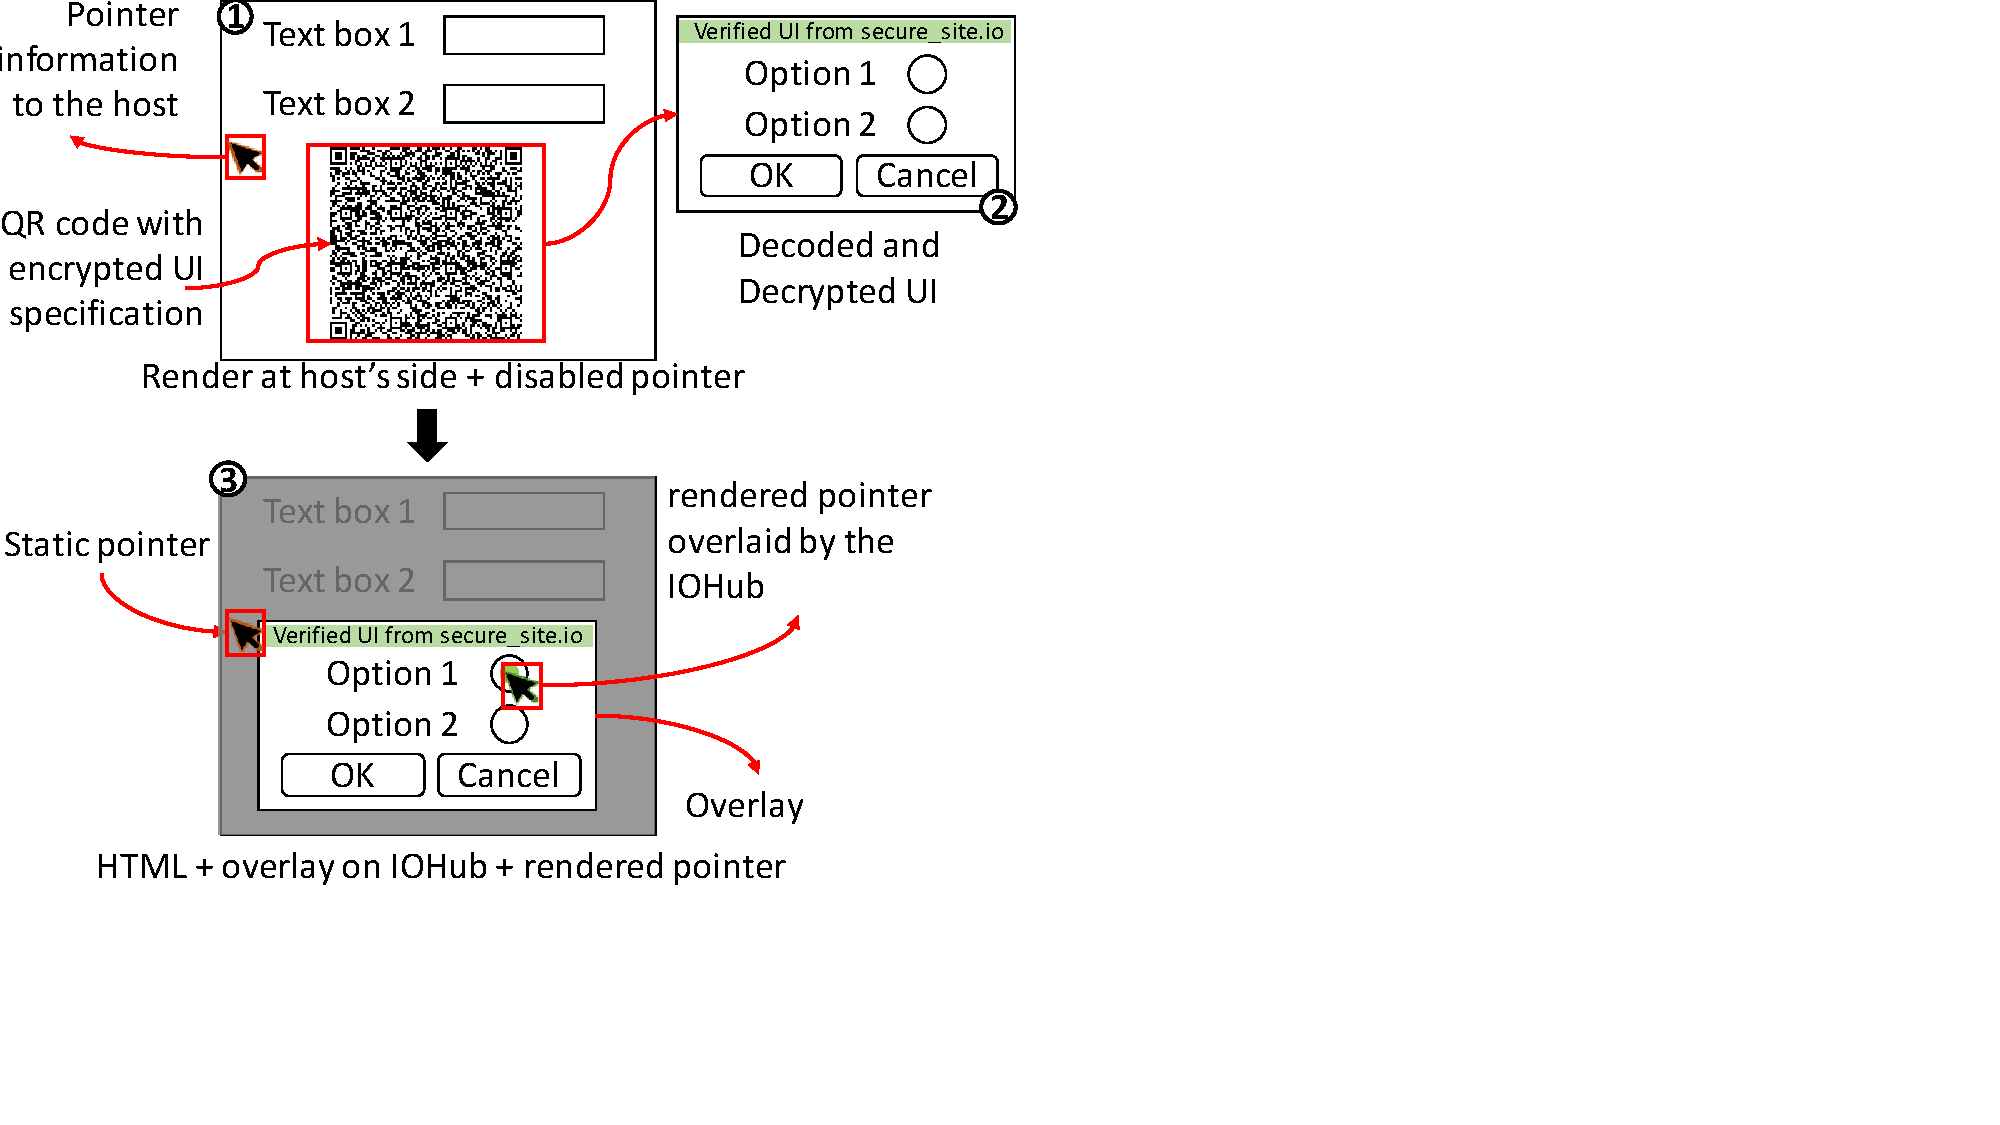
\includegraphics[trim={0 4cm 16.5cm 0}, clip, width=0.88\linewidth]{activityPrivacyRender.pdf}
%\caption{\textbf{\name IO confidentiality.} The figure shows how \name achieves the confidentiality of the UI elements and the mouse pointer in the presence of a compromised host. The upper screenshot shows the host's view of the display, while the lower one shows the user's view. The host can only see a QR code where the specification is encrypted by the \tls session key between the \device and the remote server. The user saw the decoded and overlaid UI objects that are retrieved from the QR code sent by the remote server (as described in Section~\ref{sec:systemDesign:transformation}).}
\caption{\textbf{\name IO confidentiality.} The figure shows \one the browser render of the webpage in Specification~\ref{snippet:encryptedHTML} where the \name \js produces the encrypted QR code. \two shows the UI overlay that is decrypted and decoded by the \device. \three shows the user's view when the \device overlays the UI on the HDMI frame, and the user starts to interact with the UI.}
\spacesave
\label{fig:activityPrivacy}
\centering
\end{figure}

\subsection{Focusing User Attention} 
\label{sec:confidentiality:SAS}

The IO confidentiality could be viewed as a similar problem to \emph{phishing} where the user provides the inputs to an attacker-generated UI (or a phishing webpage) that leaks the sensitive information. Similar to the phishing protection mechanisms, IO confidentiality requires additional attention/operations from the user. Secure Attention Sequence (SAS) is a sequence of trustworthy actions (such as keystrokes \texttt{Ctrl+Alt+Del} in Windows) executed by the user. SAS prevents an untrusted system from triggering an event that is otherwise sensitive to the user. Note that SAS is a well-researched topic in the context of UI/UX design. \name adapts an off-the-shelf SAS mechanism that provides a visual aid for the user to distinguish overlaid UI and the mouse pointer location. SAS is crucial for IO confidentiality as the untrusted host can trick the user into inputting her sensitive information on a forged form. Hence, the user needs to remember the SAS to distinguish \device generated UIs from host generated UIs. Note that the automated activation is insufficient as at any given time, the host can maliciously emulate the automated activation to trick the user into providing sensitive information to an illegitimate UI.

Note that, SAS is one of a ways to inform the user securely about the trusted overlay on the screen generated by the \device. Evaluation of the effectiveness of SAS over other attention focusing mechanisms is out-of-scope of this paper. Hence, \name uses SAS as an example attention focusing mechanism for confidentiality. In principle, \name could be integrated with other proposed approaches such as security indicators, or secret images~\cite{6894474,Marforio2016}.

\myparagraph{SAS policy} The remote server can set configurable SAS policy per overlaid UI (i.e., QR code). The SAS policy is defined in the \texttt{SAS} attribute in the example specification provided in Specification~\ref{snippet:UISpecification}. By default, the overlaid UI is locked from the user and requires \red{the SAS keystroke from the user to unlock the sensitive UI. This information is overlaid on the UI to remind the user to execute it. Note that we oped for a system-wide SAS as this prevents the attacker to put a fake SAS on the screen, The SAS keystroke is first intercepted by the \device that checks for the QR code on the HDMI stream. One example policy could be \texttt{5:LB} which denotes \device invokes a lightbox on the HDMI frames except for the UI overlay and the mouse pointer overlay for a specified time (here for $5$ seconds} 
%One example policy could be \texttt{Ctrl+d:5}, which denotes that the user needs to press key `\texttt{Ctrl+d}' to unlock the UI overlay. Pressing this key also triggers the \device to black out the HDMI frames except for the UI overlay and the mouse pointer overlay for a specified time (here for $5$ seconds). 


